\section{Artificial Neural Networks \label{sec: neural nets}}

    \begin{figure}[h]
        \centering
        \begin{subfigure}[b]{0.9\textwidth}
            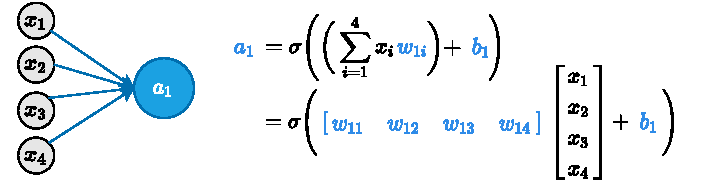
\includegraphics[width=\textwidth]{one_neuron.pdf}
            \caption{A single neuron connected to the input layer of 4 input \glspl{neuron}. It computes the activation function of the weighted sum of the previous layer's outputs as its own output. \label{subfig: neuron}}
        \end{subfigure}
        \hfill
        \begin{subfigure}[b]{0.9\textwidth}
            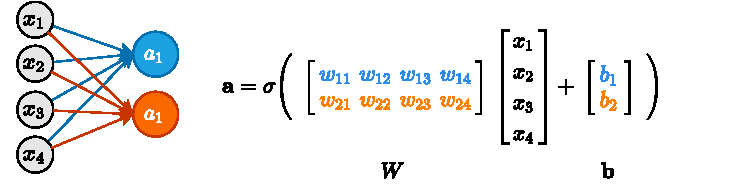
\includegraphics[width=\textwidth]{two_neurons.pdf}
            \caption{Using notation from linear algebra, the calculations computed by the whole layer (of two \glspl{neuron}) can be written as an activation function of a matrix multiplication and vector addition. \label{subfig: layer}}
        \end{subfigure}
        \caption{4 input \glspl{neuron} $x_i$ are connected to the next layer consisting of one \gls{neuron} (a) or two \glspl{neuron} (b).}
    \end{figure}

    

    The \glspl{model} used for supervised learning throughout this project are called \glspl{nn}. They are flexible information processing architectures (loosely) inspired by the network of \glspl{neuron} in the human brain.
    %It is not strictly necessary to understand the functionality of \glspl{nn} to understand the rest of the project, simply noting that \glspl{nn} are flexible functions $\hat{f}_{\theta} : X \rightarrow Y$ that can be trained to process information in the desired way using labelled training data $(X, Y)$ is enough. A quick introduction is however included for completeness.
    
    \subsection{Neurons}
        \Glspl{nn} are a collection of connected nodes called \textbf{\glspl{neuron}} that are sequentially organised into a number of layers. Each \gls{neuron} contains a set of weights $w_i$ and a set of biases $b_i$ with $i \in [1, N_{in}]$, where $N_{in}$ is the number of inputs to that \gls{neuron}. A \gls{neuron} in layer $l$ takes inputs $a_i^{(l-1)}$ from the previous layer $l-1$ and calculates its output as a weighted sum normalised by a non-linear \textit{activation function} $\sigma$ (see Sec. \ref{ssec: activation function}):
    
        \begin{equation}
            \label{eq: feed forward}
            a^{(l)} = \sigma\bigg(\big(\sum_{i = 1}^{N_{in}} w_i a_i^{(l-1)}\big) + b\bigg).
        \end{equation}
        
        This output is the input for all connected \glspl{neuron} in the next layer, hence it is equal to $a^{(l)}$. 
        %This process of processing information is called the forward pass of the \gls{nn}. 
        A simple example of a \gls{neuron} is shown in Fig. \ref{subfig: neuron}.
    
    \subsection{Layers}
        \glspl{nn} are composed of multiple layers of multiple \glspl{neuron}. In many \glspl{nn}, every \gls{neuron} in layer $l$ is connected to every \gls{neuron} in the next layer $l + 1$. We assume that this is the general case within this section. This allows for the use of linear algebra notation to simplify what each layer does.
        
        Writing the input vector of layer $l$ as $\mathbf{a}^{(l)}$, the weight matrix, containing all the weights of a \gls{neuron} (column) for all \glspl{neuron} in a layer (row) as $W$ and the vector of biases of all \glspl{neuron} in a layer as $\mathbf{b}$ allows us to write the forward pass through each layer as
        
        \begin{equation}
            \mathbf{a}^{(l)} = \sigma(W\mathbf{a}^{(l-1)} + \mathbf{b}),
        \end{equation}
        
        %as \[
        %    \sigma\bigg( \big(x_0, x_1, \dots x_n) \bigg) = \bigg( \sigma(x_0), \sigma(x_1) \dots \sigma(x_n)\bigg). %todo make col vec
        %\]
        A simple example, with only two layers can be found in Fig. \ref{subfig: layer}. The inputs to the first layer are the inputs to $\hat{f}_\theta$, $X$. The output(s) of the last layer are the predicted results $\hat{Y}$. 
        
        %The information processing of a \gls{nn} with $N$ layers can thus be written as the repeated nested application of a weighted sum normalised at every layer $j$ by some $\sigma^{(j)}$:
        %
        %\begin{align}
        %    \label{eq: nested NN}
        %    \hat{\mathbf{Y}} = \mathbf{a}^{(N - 1)} &= \sigma^{(N-1)}\bigg(W^{(N - 1)}\mathbf{a}^{(N - 2)} + \mathbf{b}^{(N-1)}\bigg) \\
        %    &= \sigma^{(N-1)}\bigg(
        %        W^{(N - 1)}\big( \dots (
        %        \sigma^{(0)} \big(
        %            W^{(0)} (\mathbf{X})) + \mathbf{b}^{(0)}
        %            \big) \dots
        %        \big) + \mathbf{b}^{(N-1)} \nonumber
        %    \bigg).
        %\end{align}
        %The weights $W$ and biases $\mathbf{b}$ determine how the inputs $\mathbf{X}$ are processed to the outputs $\mathbf{Y}$ and are the parameters $\theta$ of the \gls{model}. Framing the calculations in this way allows hardware made for parallelised computing, such as Graphical Processing Units (GPUs), to accelerate computations significantly\cite{herlihy2012art}.
        
        %It is beneficial to frame computations as linear algebra operations because of available hardware: A computer's GPU (graphical processing unit) is capable of processing large numbers of repeated calculations much faster than central processing units (CPUs), by computing all required values in parallel\cite{herlihy2012art}. 
        %Linear algebra computations (such as matrix multiplications and vector additions) are examples where highly parallel computation can accelerate computations significantly, reducing the time needed to process data using \glspl{nn} significantly.\cite{herlihy2012art}
        
        %By inspecting Eq. \ref{eq: nested NN} and noting that every $W$ is a potentially large matrix and every $\mathbf{b}$ a potentially large vector of parameters, it is clear that the number of parameters grows quickly with the complexity of the \gls{nn}'s architecture (i.e. its number of \glspl{neuron}, and number of input features $\mathbf{X}$). It is not uncommon that the number of parameters exceeds 10s of millions for complex models. The state of the art language model, known as GPT-3 uses 175 billion parameters \cite{gpt3}. Because the models use so many parameters, they are memory intensive, which is an issue we face (and overcome) due to limited resources.
        The training process, in which all parameters $W, \mathbf{b} \in \theta$ of each layer are tuned is explained in Sec. \ref{ssec: training}.
        
        %The scale of complex \glspl{nn} is also the reason why it is beneficial to frame computations as linear algebra operations: A computer's GPU (graphical processing unit) is capable of processing large numbers of repeated calculations much faster than central processing units (CPUs), by computing all required values in parallel\cite{herlihy2012art}. 
        %Linear algebra computations (such as matrix multiplications and vector additions) are examples where highly parallel computation can accelerate computations significantly, reducing the time needed to process data using \glspl{nn} significantly.\cite{herlihy2012art}
        
        \subsection{Activation Functions \label{ssec: activation function}}
    
        There are a number of different choices for the activation function $\sigma$. Most activation functions normalise values to lie within some fixed interval $(a_{min}, a_{max})$, i.e.
        \begin{equation}
        \sigma : x \rightarrow y, \hspace{3em} x \in [-\infty, \infty], y \in (a_{min}, a_{max}).
        \end{equation}
        Examples for $\sigma$ include $\tanh{x}$, $1/(1 + e^{-x})$, or the Heaviside step-function, each of which is used for different purposes.
        
        The normalisation provided by the activation function means that a small number of \glspl{neuron} can not dominate the final outcomes too heavily (known as the ``exploding gradients problem"). The second effect of these functions is the non-linearity they introduce, allowing for non-linear models for non-linear problems\cite{mlTextbook}.
        
    \subsection{Training \label{ssec: training}}
        To train the \gls{nn} is to determine a set of parameters $\theta$ that make the \gls{model} map $X \rightarrow \hat{Y}$ in such a way that matches the provided \textit{true labels} $Y$. This is approached as an optimisation problem, where the quantity minimised is called the loss\cite{mlTextbook}.
        
        \subsubsection{Loss Function}
            The loss function maps predicted labels and true labels to the so-called loss $L$: \[\mathcal{L} : \hat{Y}, Y \rightarrow L.\] $L$ is a measure of goodness of fit between the model's predictions and the true labels. One commonly used example is the mean-squared-error as the loss function:
            \begin{equation}
                \mathcal{L} = \frac{\sum_{i = 1}^{N_d}(Y_i - \hat{Y}_i)^2}{N_d}, \hspace{2em} \hat{Y}_i = \hat{f}_\theta(X_i),
            \end{equation}
            where the sum is over all $N_d$ true data points $(X_i, Y_i)$.
            Since $\hat{Y}$ depends on $\theta$, $\mathcal{L} = \mathcal{L}(\theta)$. Since $\mathcal{L}$ and $\sigma$ are both differentiable functions, partial derivatives of $\mathcal{L}$ with respect to $\theta$ can be calculated. 
        
        \subsubsection{Gradient Descent}
            By computing the gradient of $\nabla_\theta \mathcal{L}$ with respect to $\theta$, and slowly moving all weights towards the minimum along this gradient, a set of weights that minimises the $\mathcal{L}$ (and thus optimises the prediction) can be found. Writing all parameters $\theta$ as a vector $\boldsymbol{\theta}$, this gradient descent process can be written succinctly as
            
            \begin{equation}
                \boldsymbol{\theta} \rightarrow \boldsymbol{\theta} - \alpha \nabla_\theta \mathcal{L}(\boldsymbol{\theta}),
            \end{equation}
            repeated until convergence, where $\alpha \ll 1$ is the learning rate, chosen manually.